\section*{Теория}

Рассмотрим условие квазинейтральности с точки зрения средних плотностей заряда. Пусть концентрация ионов равна $n_i$, концентрация электронов -- $n_e$, и каждый ион отдаёт в плазму $Z$ электронов. Тогда условие квазинейтральности запишется в виде:
$$
-en_e + (Ze) n_i = 0, 
$$
$e > 0$ -- элементарный заряд. Далее для простоты изложения будем рассматривать случай однократно ионизованной плазмы $Z = 1$.

\subsection*{Нарушение квазинейтральности плазмы в квазиодномерном случае}

На микроуровне квазинейтральность плазмы может нарушатся из-за тепловых флуктуаций. Отклонение от квазинейтральности может происходить только на малых расстояниях и в течение малых промежутках времени. Оценим характерные расстояния, на которых может происходить разделение зарядов.

\begin{wrapfigure}{left}{0.5\textwidth}
	\vspace{-10pt}
	\centering
	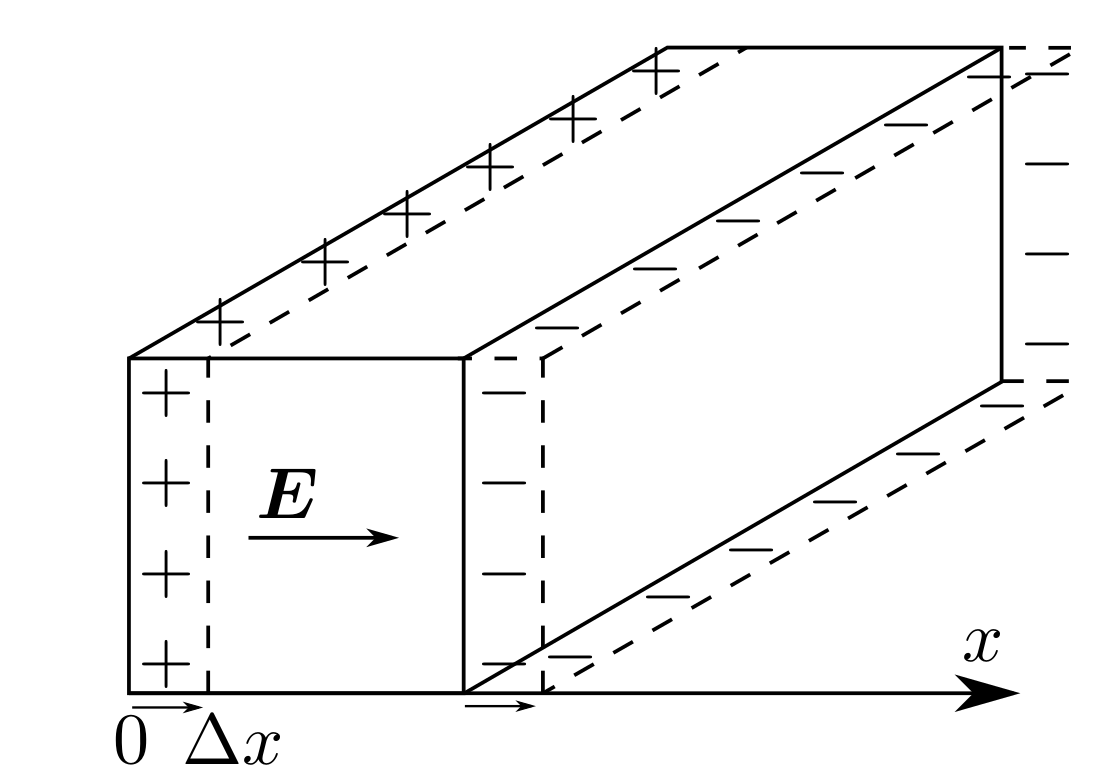
\includegraphics[width=0.48\textwidth]{../res/plasma.png}
	\caption{Плазменные колебания.}
	\label{img:plasma oscil}
\end{wrapfigure}

Пусть в некотором слое толщиной $l$ произошло разделение зарядов. В состоянии равновесия $n_i = n_e \equiv n$. В результате разделения зарядов на боковых плоскостях возникнут нескомпенсированные заряды с плотностью
$$\sigma = \frac{neV}{S} = nel$$
Выделенный слой можно рассматривать как плоский конденсатор. Напряженность электрического поля в плазме будет
$$E = 4\pi \sigma = 4\pi n el$$.
Объёмная плотность энергии такого поля равна
$$\omega_E = \frac{E^2}{8\pi}$$.
Так как электрическое поле было создано разделенными в результате тепловой флуктуации зарядами, то, согласно закону сохранения энергии, кинетическая энергия теплового движения преобразовалась в энергию электрического поля:
$$w_E = w_T$$
По теореме о равнораспределении кинетической энергии по степеням свободы, так как случай одномерный, то
$$
w_T = w_{T}^e + w_{T}^i = n \frac{kT}{2} + n\frac{kT}{2} = nkT
$$
Тогда напряженность поля
$$
E = \sqrt{8nkT}
$$
и толщина слоя
$$
l = \sqrt{\frac{kT}{2\pi n e^2}}
$$
Величину $r_D = \frac{l}{2} = \sqrt{\frac{kT}{8\pi n e^2}}$ называют \textit{дебаевским радиусом} или \textit{дебаевской длиной}. 

Оценим характерное время, в течение которого может происходить разделение зарядов. Рассмотрим смещение $l$ зарядов в слое плазмы (рис. \ref{img:plasma oscil}). На электроны действует электрическое поле:
$$
E = 4 \pi n e l
$$
Запишем уравнение движения электронов:
$$m \ddot{l} = -4 \pi n e^2 l$$
Это уравнение, решением которого является гармонический осциллятор с частотой $\omega_p = \sqrt{\frac{4\pi n e^2}{m}}$, называемой \textit{ленгмюровской} или \textit{плазменной}. 

Таким образом, ленгмюровская частота $\omega_p$ определяет время отклика плазмы на флуктуацию заряда, а дебаевский радиус определяет характерные размеры флуктуаций. То есть ленгмюровская частота и дебаевский радиус характеризуют временной и пространственный масштаб плазменных явлений.

Теперь можно дать количественное описание коллективного характера взаимодействия плазмы. Плазмой можно считать газ, дебаевский радиус которого много меньше характерного размера области $d$, занимаемой газом:
$$
r_D = \sqrt{\frac{kT}{8 \pi n e^2}} \ll d
$$
Если характерный размер области меньше дебаевского радиуса, то тепловые флуктуации будут оказывать более значительное влияние, чем электромагнитные взаимодействия. Тогда можно будет рассматривать только взаимодействия частиц во время столкновений, а дальнодействующими силами пренебречь.

\subsection*{Плазменное экранирование}

Внесем в плазму точеный заряд $q$. Под действием внешнего поля электроны в плазме перераспределяться так, чтобы скомпенсировать поле точеного заряда. Из-за наличия тепловых флуктуаций полной нейтрализации поля заряда наблюдаться не будет. Ослабление внешнего поля в плазме называется \textit{экранированием}.

Потенциал точечного заряда равен
$$\varphi_q = \frac{q}{r}$$
Распределение заряженных частиц в электрическом поле определяется распределением Больцмана:
$$
n_e = n e^{\frac{e \varphi}{kT}}, \hspace{2mm} n_i = n e^{-\frac{e \varphi}{kT}}
$$
На бесконечности потенциал поля будет равен нулю, и в силу квазинейтральности концентрации электронов и ионов будут равны.

Получим выражение объемной плотности заряженных частиц в плазме используя распределение Больцмана. Считая точечный заряд, а следовательно и его потенциал, малым по величине разложим экспоненту по формуле Тейлора.
$$\rho = -e n_0 + e n-i = en \left( e^{-\frac{e\varphi}{kT}} - e^{\frac{e \varphi}{kT}} \right) \approx \frac{-2 ne^2}{kT} \varphi$$
Распределение потенциала электрического поля определяется уравнением Пуассона:
$$
\nabla^2 \varphi = - 4 \pi \rho
$$
Поле точечного заряда имеет сферическую симметрию, тогда уравнение Пуассона представимо в виде:
$$
\frac{1}{r}\frac{d^2(r \varphi)}{d r^2} = \frac{8 \pi n e^2}{kT} \varphi
$$
На малых расстояниях от точечного заряда суммарный потенциал примерно равен потенциалу точечного заряда $\phi_q$. Тогда итоговым распределением потенциала будет
$$
\varphi = \frac{q}{r} \exp \left( -\frac{r}{r_D} \right)
$$
Этот потенциал называется \textit{дебаевским потенциалом}.

Оценим энергию кулоновского взаимодействия частиц в плазме. Ионы считаем однозарядными. Представим плазму в следующем виде: ионы будут положительными точечными пробными зарядами, помещенные в плазму, электроны будут их экранировать. В результате суммарное электрическое поле в плазме будет отсутствовать. Будем считать, что ионы между собой не взаимодействуют, и также не взаимодействуют между собой электронные облака, экранирующие разные ионы. Тогда энергия плазмы равна работе, которую необходимо затратить, чтобы поместить вокруг ионов электронные облака, то есть равна сумме потенциалов электронных облаков, количество которых равно числу ионов в плазме. Потенциал экранирующего облака равен
$$
\varphi_{обл} = \varphi_{деб} - \varphi_{ион} = \frac{e}{r} \left(\exp \left( -\frac{r}{r_D} \right) - 1\right) \approx - \frac{e}{r_D}
$$
Электростатическая энергия системы зарядов вычисляется по формуле $W = \frac{1}{2} \sum_n (\varphi_n q_n)$. Тогда объемная энергия плазмы равна
$$
\omega = - \frac{1}{2} n_i \frac{e^2}{r_D}
$$

\subsection*{Идеальная и не идеальная плазмы}

Рассмотрим \textit{дебаевскую сферу} -- область в плазме, ограниченную сферой радиуса $r_D$. Концентрация частиц в сфере
$$
N = \frac{4}{3} \pi r_D^3 n
$$
В веществе объемом $V$ и концентрацией частиц $n$ находится $N = nV$ частиц, тогда каждая частица в среднем занимает объем $V_0 = \frac{V}{N} = \frac{1}{n} \sim d^3$, поэтому среднее расстояние между частицами $d \sim n^{-1/3}$. Тогда 
$$N \sim \left( \frac{r_d}{d} \right)^3$$

Рассмотрим два предельных случая.
\begin{enumerate}
	\item $N \gg 1$. То есть в дебаевской сфере находится очень много частиц. Так как экранирование на расстояниях порядка дебаевского радиуса $r_D$ невелико, то заряженные частицы будут проявлять коллективные эффекты, связанные с электромагнитным взаимодействием. Заметим, что хотя количество частиц в сфере велико, плазма является \textit{разреженной} из-за большого дебаевского радиуса:
	$$
	r_D \sim \sqrt{\frac{kT}{8 \pi n e^2}} \gg n^{-1/3} \Rightarrow n \ll \left( \frac{kT}{e^2} \right)^3
	$$
	Покажем, что потенциальная энергия взаимодействия частиц мала по сравнению с их кинетической энергией. Условие разреженной плазмы можно переписать в виде:
	$$w_E \sim \frac{e^2}{d} \ll w_T \sim kT$$
	Плазму называют \textit{идеальной}, если потенциальная энергия взаимодействия частиц мала по сравнению с кинетической энергией. В данном случае плазму с хорошей точностью можно рассматривать как идеальный газ.
	
	\item $N \ll 1$. Из-за малого дебаевского радиуса, плотность плазмы велика:
	$$n \gg \left( \frac{kT}{e^2} \right)^3$$
	Такую плазму называют \textit{плотной}, и её нельзя рассматривать как идеальный газ.
\end{enumerate}

\subsection*{Квазиравновесная плазма}

Плазма может находится квазиравновесном состоянии, когда температуры электронов и ионов отличаются на порядки. Пусть сначала скорости электронов и ионов распределены изотропно, но не удовлетворяют максвелловскому распределению скоростей. Тогда из-за различия масс электронов и ионов сначала установится максвелловское распределение скорости электронов, затем ионов. При этом температура электронов не обязательно будет равна температуре ионов $T_e \neq T_i$, такую плазму называют \textit{неизотермической} или \textit{двухтемпературной}. Затем в результате взаимодействия электронов и ионов установится максвелловское распределение скоростей для всей плазмы (\textit{изотермическая плазма}).

Если плазма находится в электрическом поле, то в ней течет электрический ток. Энергию от поля получают в основном электроны, так как они более подвижные. Ионы получают основную энергию за счет взаимодействия с быстрыми электронами. В итоге, так как ионы нагреваются достаточно медленно, различие температур электронов и ионов может составлять несколько порядков.

\subsection*{Плавающий потенциал}

Для исследования свойств плазмы используется зондовый метод. Зонд, представляющий собой небольшой проводник, помещается в плазму и измеряет электрический потенциал. Измерив вольт-амперную характеристику зонда, можно определить температуру плазмы, её дебаевский радиус и ленгмюровскую частоту.

\begin{wrapfigure}{left}{0.5\textwidth}
	\vspace{-10pt}
	\centering
	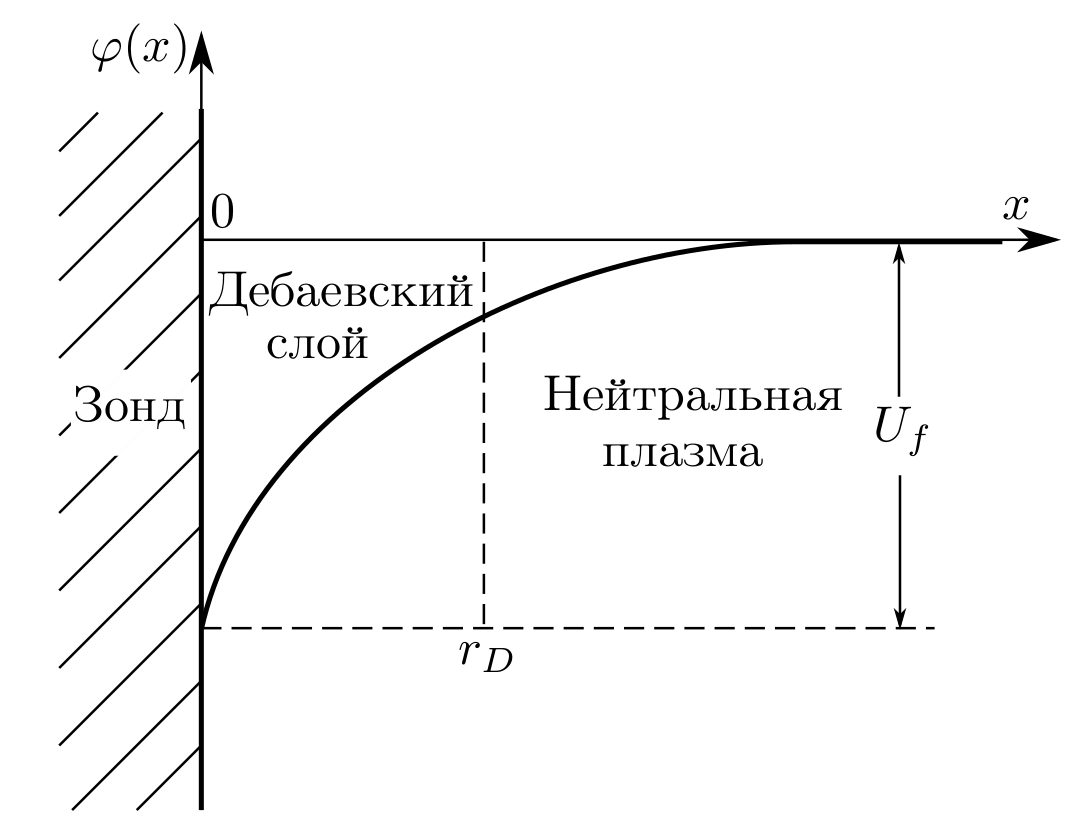
\includegraphics[width=0.48\textwidth]{../res/probe.png}
	\caption{Плавающий потенциал.}
	\label{img:plasma probe}
\end{wrapfigure}

При внесении проводника в плазму он подвергается бомбардировке заряженными частицами, преимущественно электронами. Будем считать плазму идеальной. Тогда поток электронов на единичную поверхность равен:
$$
j = \frac{1}{4} n \bar v
$$
где $\bar v = \sqrt{\frac{8 k T}{\pi m}}$ -- средняя тепловая скорость движения частиц. Так как скорость электронов больше скорости ионов, то проводник зарядится отрицательно и приобретет отрицательный потенциал $-U_f$, называемый \textit{плавающим потенциалом}.

В начальный момент времени потенциал зонда равен $0$, тогда электронный и ионный токи, которые называют \textit{тепловыми} равны:
$$
I_{e0} = -\frac{n \bar v_e}{4} eS, \hspace{2mm} I_{i0} = \frac{n \bar v_i}{4} eS
$$
Когда потенциал зонда станет равен $-U_f$, то электроны будут замедляться зондовым полем, ионы ускорятся. Так как масса ионов большая, то потенциальный барьер зонда практически не повлияет на ионный ток:
$$
I_i \approx I_{i0}
$$
Электронный ток уменьшится, так как только электроны обладающие достаточной кинетической энергией способны преодолеть потенциальный барьер. Так как распределение электронов по энергии определяется распределением Больцмана, то электронный ток равен
$$
I_{e} = I_{e0} \exp \left( -\frac{e U_f}{kT_e} \right)
$$
В состоянии равновесия электронный и ионный токи равны $I_e = I_i$. Тогда
$$
U_f = -\frac{kT}{e} \ln{\frac{\bar v_i}{\bar v_e}} = \frac{1}{2} \frac{kT}{e} \ln{\frac{T_e m_i}{T_i m_e}}
$$

\subsection*{Измерение с помощью двойного зонда}

\textit{Двойным зондом} называется система, состоящая из двух зондов, расположенным на небольшом расстоянии друг от друга. Между зондами создаётся разность потенциалов $U$, которая по величине много меньше плавающего потенциала. При этом оба зонда имеют близкий к плавающему потенциалу потенциал.
\begin{equation*}
	\begin{split}
		U_1 &= U_f + \Delta U_1 \\
		U_2 &= U_f + \Delta U_2
	\end{split}
\end{equation*}
Где $U_1$ -- потенциал первого зонда, $U_2$ -- потенциал второго зонда, $\Delta U_1, \Delta U_2 \ll U_f$.
$$
U = \Delta U_2 - \Delta U_1
$$

\begin{wrapfigure}{left}{0.5\textwidth}
	\vspace{-10pt}
	\centering
	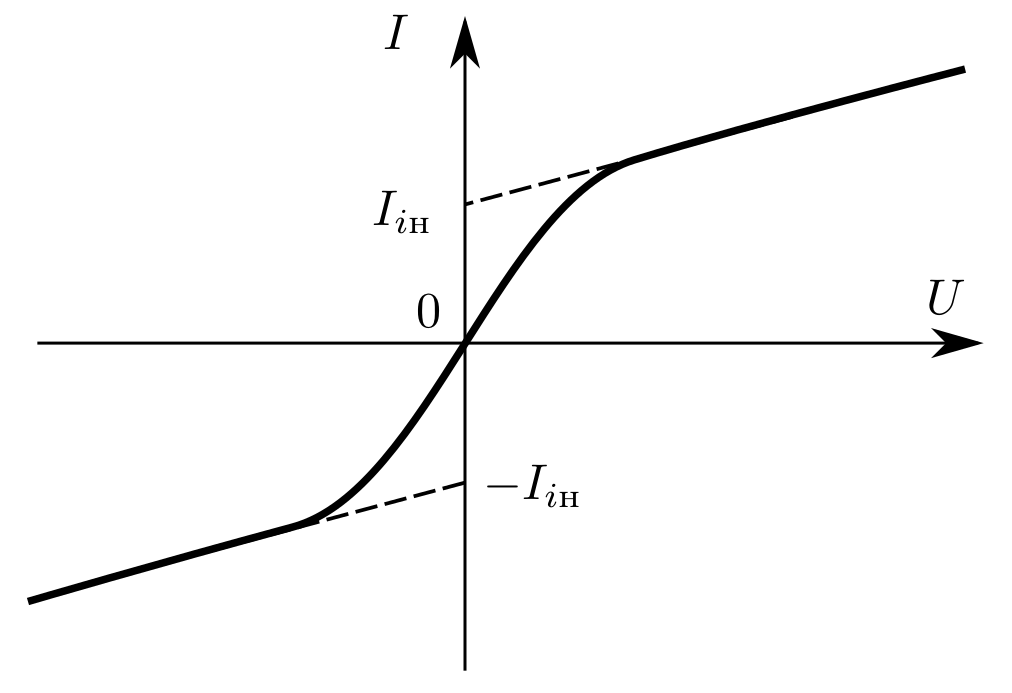
\includegraphics[width=0.48\textwidth]{../res/two probes.png}
	\caption{Плавающий потенциал.}
	\label{img:plasma two probes}
\end{wrapfigure}

Вольт-амперная характеристика зонда представлена на рисунке \ref{img:plasma two probes}. \textit{Током насыщения} называется ток, которому соответствует точка пересечения наклонной асимптоты и оси ординат. На левой ветви в пределе $U \rightarrow - \infty$ электронный ток прекращается $I_e \rightarrow 0$, на правой ветви  $U \rightarrow \infty$ прекращается ионный ток из-за потенциального барьера. Электронный ток насыщения можно оценить по формуле
$$
I_{eн} \approx I_{e0} \approx \frac{1}{4} n_e S \sqrt{\frac{8 kT}{\pi m_e}}
$$
Для ионного тока такая оценка слишком груба, поэтому применяется полуэмпирическая формула Д. Бома:
$$
I_{iн} \approx 0,4 n_i eS \sqrt{\frac{2 kT_e}{m_i}}
$$
Приближенная зависимость, описывающая вольт-амперную характеристику двойного зонда:
$$
I = I_{i н} \th \left( \frac{eU}{2 kT_e} \right)
$$
Данная зависимость не учитывает наклонные асимптоты графика и с достаточной точностью применима при $|U| < |U_f|$.